%------------------------------------------------------------------%
% Cannabis Data Science Presentation
%------------------------------------------------------------------%
\documentclass[xcolor={dvipsnames}]{beamer}
\hypersetup{pdfpagemode=FullScreen}
\mode<presentation> %TEMPLATE
{ \usetheme{Boadilla}
  \usecolortheme{orchid}
  \usefonttheme{default}
  \setbeamertemplate{navigation symbols}{}
  \setbeamertemplate{caption}[numbered]} 
\usepackage[english]{babel}
\usepackage[utf8x]{inputenc}
\setbeamersize{text margin left=0.5in,text margin right=0.5in}

\definecolor{myNewColorA}{rgb}{2,48,32}
\definecolor{myNewColorB}{rgb}{0,100,100}
\definecolor{myNewColorC}{rgb}{0,200,100}
\definecolor{myNewColorD}{rgb}{0,100,200}

%\setbeamercolor*{palette primary}{bg=myNewColorA, fg = white}
%\setbeamercolor*{palette secondary}{bg=myNewColorB, fg = green}
%\setbeamercolor*{palette tertiary}{bg=myNewColorC, fg = green}
%\setbeamercolor*{palette quaternary}{bg=myNewColorD, fg = green}
%------------------------------------------------------------------%
% Packages
%------------------------------------------------------------------%
\usepackage{amsmath}
\renewcommand*\footnoterule{} %No sperating line on footnote
\usepackage{mathtools} %ANNOTATING EQUATIONS
\usepackage{hhline} %DOUBLBARS
\newcommand\T{\rule{0pt}{2.5ex}} %TOPSTRUT
\newcommand\B{\rule[-1.25ex]{0pt}{0pt}} %BOTTOMSTRUT
\newenvironment<>{varblock}[2][.9\textwidth] %RESIZED BLOCKS
  {\setlength{\textwidth}{#1}
  \begin{actionenv}#3
    \def\insertblocktitle{#2}\par
    \usebeamertemplate{block begin}}
  {\par\usebeamertemplate{block end}
  \end{actionenv}}
\defbeamertemplate{enumerate item}{largeball} %LARGE BALLS
{\begin{pgfpicture}{-1ex}{-0.65ex}{1.5ex}{1.5ex}
\usebeamercolor[fg]{item projected}
{\pgftransformscale{2.5}\pgftext{\Large\pgfuseshading{bigsphere}}}
{\pgftransformshift{\pgfpoint{0pt}{0.5pt}}
\pgftext{\usebeamerfont*{item projected}\small\insertenumlabel}}
\end{pgfpicture}}
\usepackage{tikz} % FANCY ARROWS
\usepackage{xparse}
\NewDocumentCommand\UpArrow{O{2.0ex} O{black}}{%
   \mathrel{\tikz[baseline] \draw [->, line width=0.5pt, #2] (0,0) -- ++(0,#1);}} % FANCY UPARROW
\NewDocumentCommand\DownArrow{O{2.0ex} O{black}}{%
   \mathrel{\tikz[baseline] \draw [<-, line width=0.5pt, #2] (0,0) -- ++(0,#1);}} % FANCY DOWNARROW
%\vskip 1cm
\makeatletter
\newcommand{\LeftEqNo}{\let\veqno\@@leqno}%LEFT EQUATION #'s
\makeatother
%------------------------------------------------------------------%
% Title
%------------------------------------------------------------------%
\title[Meetup]{}
\author{Cannabis Data Science}
\institute[]{\Large Meetup}
\date{March 10, 2021}
\begin{document}
\begin{frame}{}
  \titlepage
\end{frame}
%------------------------------------------------------------------%
% Introduction
%------------------------------------------------------------------%
\section{Introduction}
\begin{frame}{}
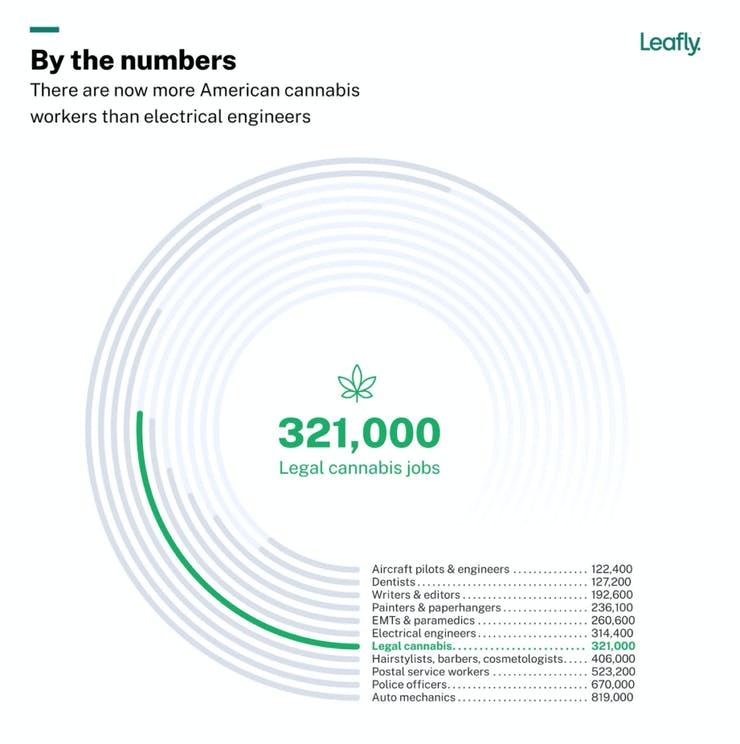
\includegraphics[scale=0.3]{images/leafly-growth-in-cannabis-jobs.png}
\end{frame}
%------------------------------------------------------------------%
% Objective
%------------------------------------------------------------------%

%------------------------------------------------------------------%
% Objective
%------------------------------------------------------------------%
\section{Charts}

\begin{frame}{}
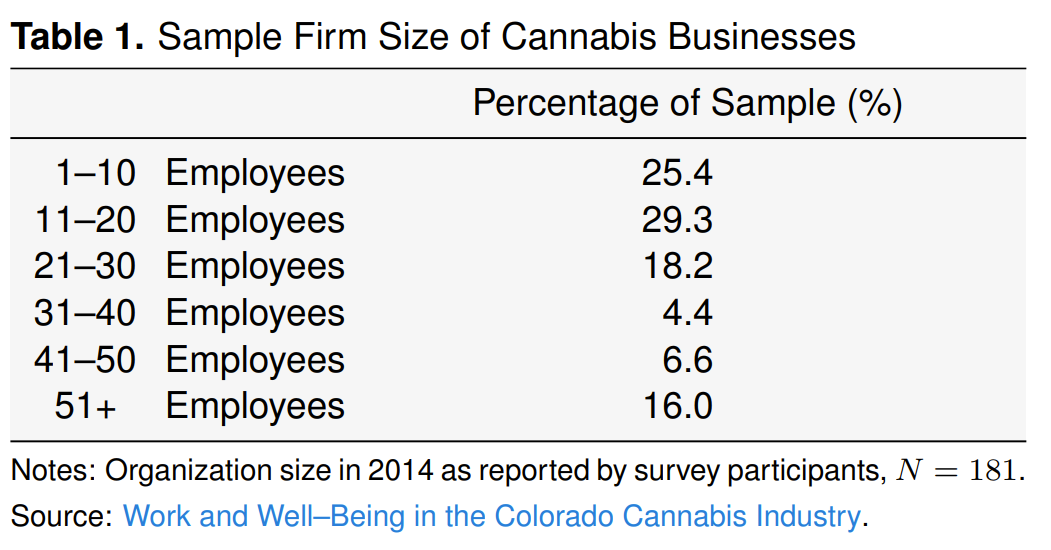
\includegraphics[scale=0.6]{images/firm-size.png}
\end{frame}

\begin{frame}{}

{Growth of Occupational Licenses} \\ {\scriptsize (Month--over--Month Percentage Change)}
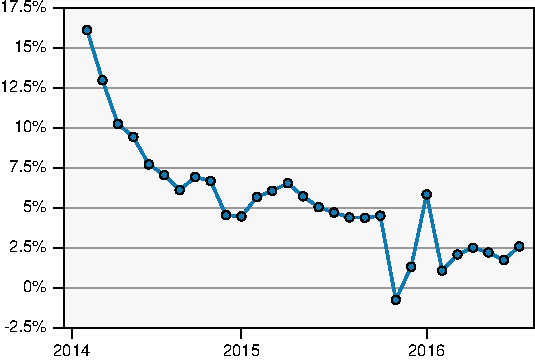
\includegraphics[scale=0.75]{images/employee_growth_plot.pdf}\\
{\scriptsize Data Source: MED 2014-2016 Annual/Mid-Year Updates.}
\end{frame}

\begin{frame}{}
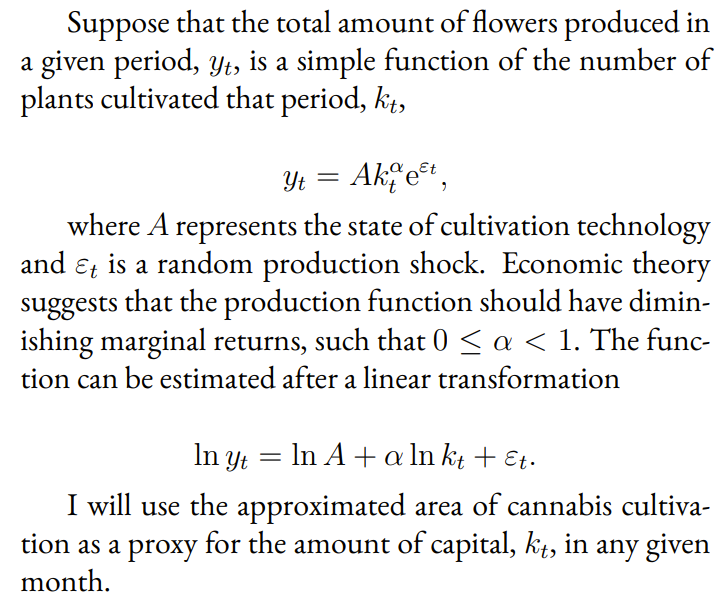
\includegraphics[scale=0.75]{images/production.png}
\end{frame}

\begin{frame}{}
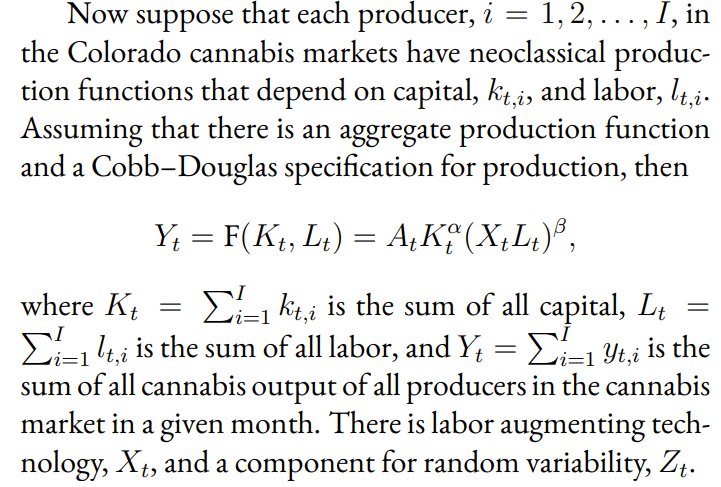
\includegraphics[scale=0.75]{images/labor.png}
\end{frame}

\begin{frame}{}
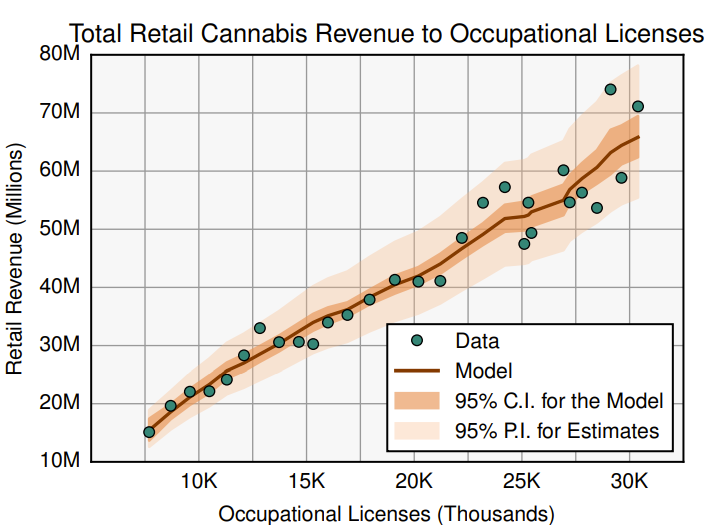
\includegraphics[scale=0.75]{images/rec-function.png}
\end{frame}

\begin{frame}{}
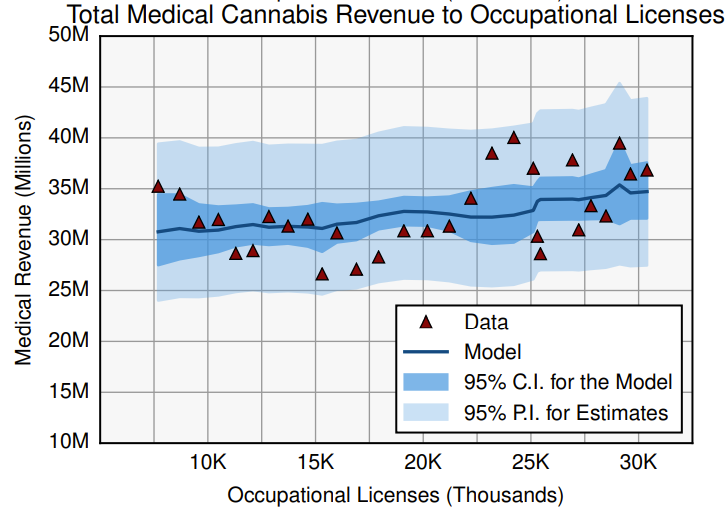
\includegraphics[scale=0.75]{images/med-function.png}
\end{frame}

\begin{frame}{}
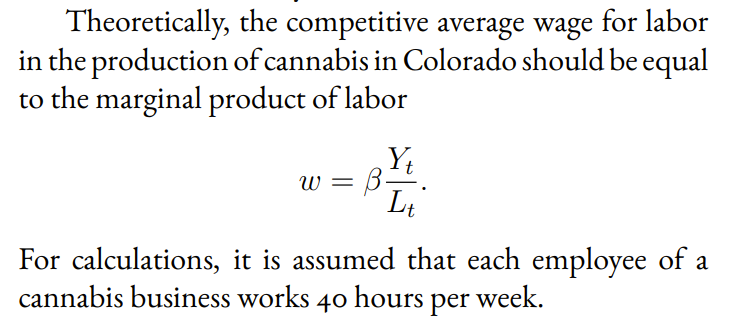
\includegraphics[scale=0.75]{images/wage.png}
\end{frame}

\begin{frame}{}
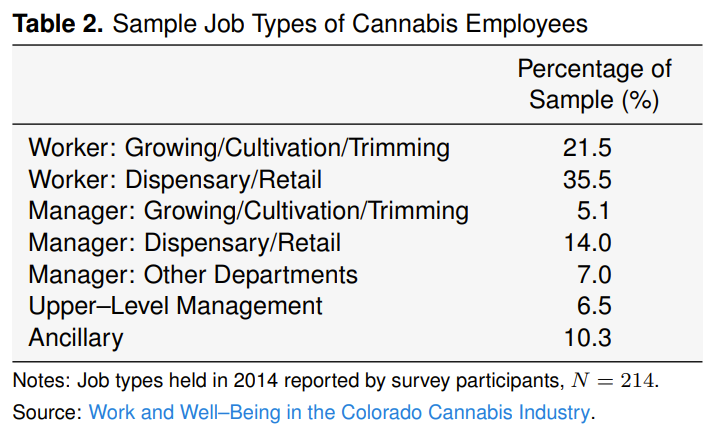
\includegraphics[scale=0.75]{images/jobs.png}
\end{frame}


%------------------------------------------------------------------%
% Takeaway
%------------------------------------------------------------------%
\begin{frame}{}
\begin{center}
\begin{minipage}{3.85in}
Thank you for coming.
\end{minipage}\end{center}
\end{frame}
%----------------------------------------------------------------%
\end{document}
%------------------------------------------------------------------%
%------------------------------------------------------------------%
%------------------------------------------------------------------%




%\only<3>{\begin{table}
%\centering
%\begin{tabular}{lc}
%\hhline{==}
%\multicolumn{2}{c}{\large \textbf{Percent of Donations Itemized}\T}\\
%\hline \T
%\large \hspace{4ex} Overall & $68\%$ \B \\
%\footnotesize \hspace{5.5ex} \textit{By family income:} & \footnotesize \\
%\small \hspace{5ex} Greater than $\$250,000$ &  $105\%$ \\
%\small \hspace{5ex} $\$100,000$ to $\$250,000$ &  $117\%$ \\
%\small \hspace{5ex} $\$60,000$ to $\$99,999$ &  $67\%$ \\
%\small \hspace{5ex} $\$25,000$ to $\$59,999$ &  $67\%$ \\
%\small \hspace{5ex} Less than $\$25,000$ &  $28\%$ \\
%\hline
%\end{tabular}
%\end{table}}